\chapter{Preliminaries}

\section{Motivation} Engineering has become a cornerstone for addressing global health and education challenges, as highlighted by UNESCO’s report \emph{Engineering for Sustainable Development} (2021), which places the discipline at the heart of the 2030 Agenda. In particular, \gls{sdg3} (“ensure healthy lives and promote well-being for all at all ages”) calls for accessible and affordable technologies to strengthen diagnostics, prevention, and healthcare delivery, while \gls{sdg4} emphasizes inclusive, equitable, and lifelong learning opportunities~\cite{nair2021engineering,de2018agenda}. Within this global framework, \glspl{bci} have gained increasing attention due to their potential to transform human–machine interaction in clinical, rehabilitative, and educational domains. Beyond their scientific and social relevance, \glspl{bci} also present growing economic impact: the global BCI market is projected to reach USD~2.21~billion by 2025 and USD~3.60~billion by 2030, with a compound annual growth rate of 10.29\%~\cite{mordor2025bci}. \glspl{bci} rely on different neurophysiological and neuroimaging technologies to capture brain activity. These include invasive approaches such as \gls{ecog}~\cite{leuthardt2004ecog}, as well as non-invasive modalities such as \gls{mri}~\cite{logothetis2008fmri}, \gls{fmri}~\cite{logothetis2008fmri}, \gls{meg}~\cite{hamalainen1993meg}, \gls{fnirs}~\cite{naseer2015fnirs}, and \gls{eeg}~\cite{vidaurre2011brain}. Each technology presents distinct trade-offs in terms of spatial and temporal resolution, portability, cost, and user comfort. While \gls{fmri} and \gls{meg} offer high spatial resolution, they are expensive, immobile, and sensitive to motion, limiting their use in real-world and longitudinal applications~\cite{logothetis2008fmri}. In contrast, \gls{eeg} provides a favorable balance between cost, portability, temporal resolution, and safety, making it particularly suitable for scalable \gls{bci} systems in clinical, educational, and community settings~\cite{chaudhary2025noninvasive}. A comparative overview of these neuroimaging and neurophysiological technologies, together with their main trade-offs in terms of invasiveness, cost, portability, and spatial--temporal resolution, is illustrated in Figure~\ref{fig:Motivation2}.

%% Figure suggestion:
%% A comparative schematic summarizing BCI technologies (EEG, fMRI, MEG, fNIRS, ECoG),
%% highlighting cost, invasiveness, spatial/temporal resolution, and portability.
\begin{figure}[h]
    \centering
    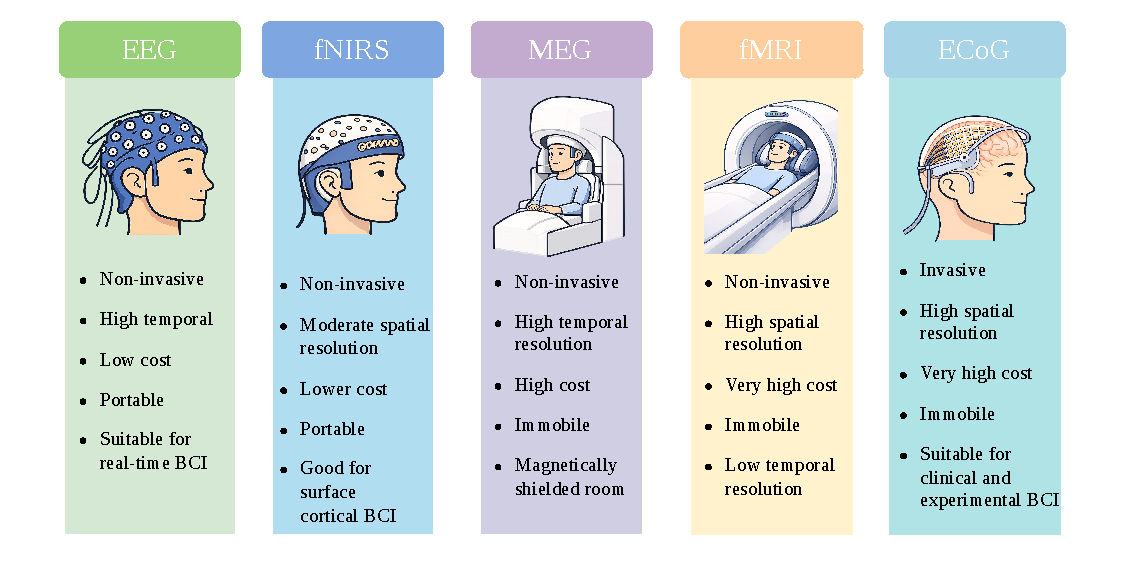
\includegraphics[width=\linewidth]{Figures/Motivacion 2.pdf}
    \caption{Overview of \gls{bci} acquisition technologies, including invasive and non-invasive modalities (\gls{eeg}, \gls{fnirs}, \gls{meg}, \gls{fmri}, and \gls{ecog}), highlighting their main trade-offs in terms of invasiveness, cost, portability, and spatial--temporal resolution.}
    \label{fig:Motivation2}
\end{figure}

In this context, \gls{eeg} has consolidated itself as a foundational technology for \gls{bci} implementation. \gls{eeg} captures electrical brain activity through scalp-mounted electrodes and enables the analysis of neural dynamics with millisecond-level temporal resolution. These characteristics support the extraction of \gls{erp} and other neurophysiological markers widely used to assess cognitive and motor functions~\cite{electronics14153106}. As a result, \gls{eeg} has become the technological backbone of many modern \gls{bci} platforms, enabling the decoding of neural activity to control external devices without requiring muscular involvement~\cite{lionakis2023trends}. Among the available paradigms, \gls{mi}—the mental rehearsal of movement without physical execution—has demonstrated notable clinical potential in post-stroke rehabilitation, neuroprosthetic control, and assistive technologies such as robotic wheelchairs and virtual spelling systems~\cite{s23052798}. Figure~\ref{fig:Motivation1} provides an overview of the conventional \gls{eeg}-based \gls{bci} pipeline, illustrating the main processing stages from signal acquisition and preprocessing to feature extraction, classification, and control or feedback generation.

\begin{figure}[H]
    \centering
    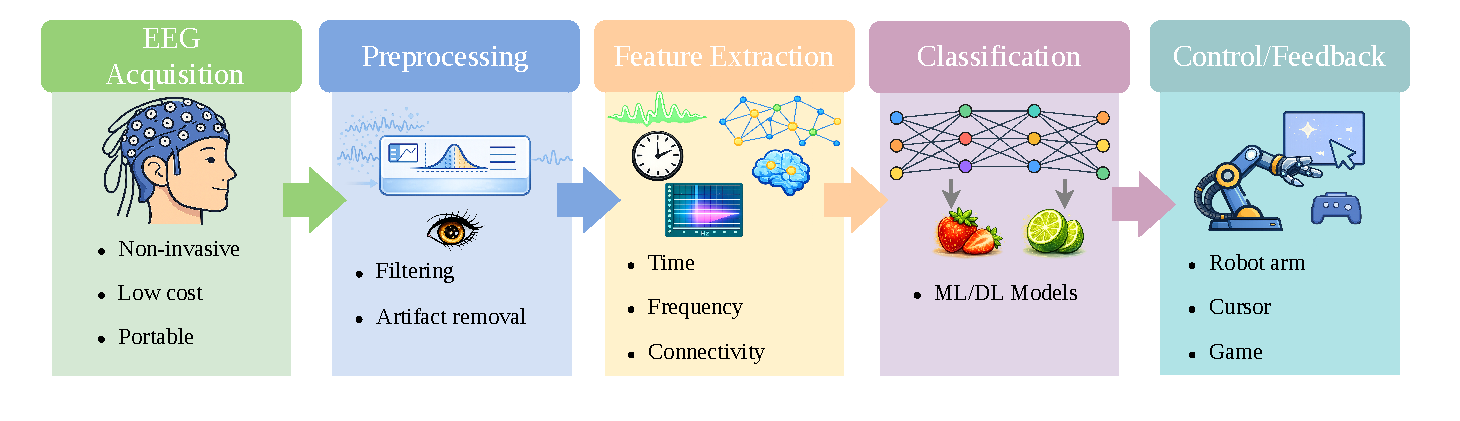
\includegraphics[width=\linewidth]{Figures/Motivation 1.pdf}
    \caption{Conventional \gls{eeg}-based \gls{bci} pipeline, illustrating the main stages from signal acquisition and preprocessing to feature extraction, classification, and control or feedback generation.}
    \label{fig:Motivation1}
\end{figure}

Beyond healthcare, \glspl{bci} have also demonstrated significant impact in educational and inclusion-oriented applications. In this context, Figure~\ref{fig:MI-TDHA} illustrates the two primary \gls{eeg} application paradigms addressed in this doctoral research, namely Motor Imagery--based
\gls{bci} decoding and \gls{eeg}-based \gls{adhd} detection. Studies report improvements in concentration, attentional focus, and engagement~\cite{djamal2020brain}, as well as promising results in the assessment and support of \gls{adhd}~\cite{maya2022hmm}. Moreover, \glspl{bci} have been integrated into pedagogical contexts to foster language comprehension and cognitive training in both children and older adults~\cite{bonnet2022kinesthetic}. These developments reinforce the societal value of \glspl{bci} by connecting health-oriented objectives (\gls{sdg3}) with education-oriented goals (\gls{sdg4}), underscoring the importance of affordable, scalable, and culturally adaptable neurotechnologies for diverse populations~\cite{nair2021engineering,de2018agenda}.

\begin{figure}[h]
    \centering
    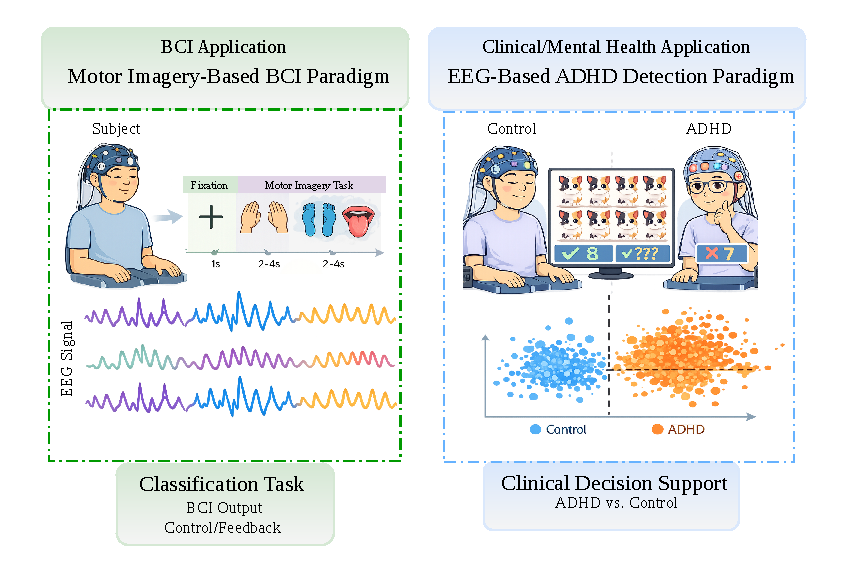
\includegraphics[width=\linewidth]{Figures/MI-TDHA.pdf}
    \caption{Overview of the two primary \gls{eeg} application paradigms addressed in this doctoral research. 
    Left: \gls{mi}--based \gls{eeg} \gls{bci} paradigm, where a subject performs imagined motor tasks and the resulting \gls{eeg} signals are used for classification and control or feedback generation. 
    Right: \gls{eeg}-based \gls{adhd} detection paradigm, where brain activity recorded during attention-demanding cognitive tasks is analyzed to support clinical decision-making by distinguishing between \gls{adhd} and control subjects.}
    \label{fig:MI-TDHA}
\end{figure}

The rapid advancement of \gls{ai} and \gls{ml} has further strengthened the development of \gls{bci} systems~\cite{lotte2018review}. By enabling data-driven modeling of complex neural dynamics, AI-based approaches have expanded the capacity of \glspl{bci} to learn discriminative patterns directly from neurophysiological signals~\cite{craik2019deep}. Deep learning architectures, representation learning strategies, and adaptive models have become central components of modern \gls{bci} pipelines, allowing systems to evolve beyond handcrafted features toward more flexible and autonomous solutions~\cite{schirrmeister2017deep,roy2019deep}. Figure~\ref{fig:Motivation3} provides an overview of the integration of \gls{ai} and \gls{ml} within the \gls{eeg}-based \gls{bci} pipeline, emphasizing data-driven representation learning, adaptive modeling, interpretability, and decision-making processes.

\begin{figure}[H]
    \centering
    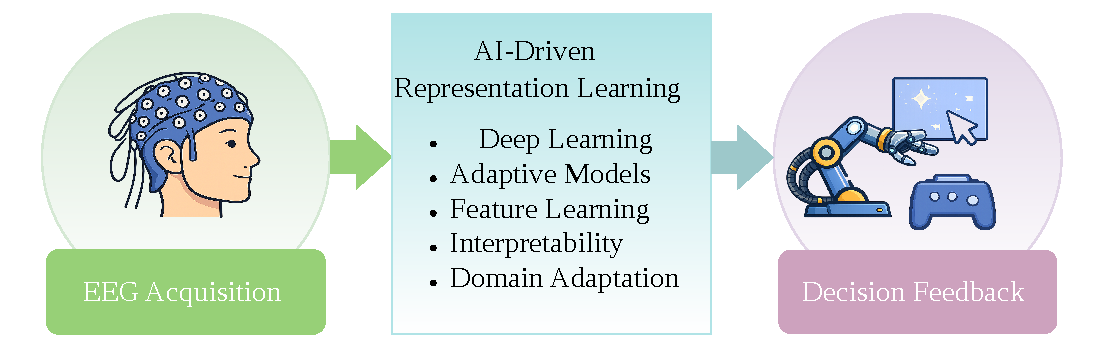
\includegraphics[width=\linewidth]{Figures/Motivation 3.pdf}
    \caption{Integration of \gls{ai} and \gls{ml} within \gls{eeg}-based \gls{bci} systems, emphasizing data-driven representation learning, adaptive modeling, interpretability, and decision-making processes.}
    \label{fig:Motivation3}
\end{figure}

The convergence of \gls{ai} and \gls{bci} technologies has opened new opportunities for the diagnosis, monitoring, and treatment of neurological and neurodevelopmental conditions~\cite{Kaboodvand2020ADHDNetworks,Shao2018ADHD}. In particular, data-driven \glspl{bci} have been explored as complementary tools for characterizing brain dynamics associated with cognitive deficits and for supporting personalized assessment and longitudinal monitoring~\cite{Kaboodvand2020ADHDNetworks}. Among these conditions, \gls{adhd} represents a pressing applied challenge, as objective and adaptive tools are required to better characterize attention, impulsivity, and hyperactivity across developmental stages~\cite{Shao2018ADHD}. Evidence further suggests that \glspl{bci}, perceptual technologies, and serious games can enhance engagement and adherence during both assessment and intervention, complementing traditional clinical and educational practices~\cite{maya2022hmm}. In this context, AI-driven \gls{eeg} analysis offers a promising avenue to support more objective, interpretable, and scalable approaches for \gls{adhd}-oriented assessment and monitoring~\cite{Kaboodvand2020ADHDNetworks}.

Addressing these emerging needs requires sustained methodological development grounded in both signal processing and \gls{ml} expertise. In response to these societal and technological needs, the \gls{gcpds} at the Universidad Nacional de Colombia has developed a sustained research line focused on neurophysiological signal analysis and the design of \gls{ml} methodologies for diagnosis, monitoring, and cognitive decoding based on \gls{eeg} data. Early contributions from the group explored kernel-based learning strategies to enhance the discrimination of neurophysiological patterns in biomedical signals, establishing a foundation for robust \gls{eeg}-based classification frameworks~\cite{Cardenas2017Kernel,Cardenas2017Enhanced}. These approaches emphasized the importance of capturing nonlinear relationships in brain signals while preserving interpretability and computational efficiency.

Building upon this foundation, subsequent work from \gls{gcpds} extended these methodologies toward clinical and applied scenarios, including cognitive assessment and neurological condition monitoring. In particular, adaptive \gls{ml} models were proposed to address variability across subjects and sessions in real-world settings, reinforcing the relevance of data-driven \gls{eeg} analysis for diagnosis and monitoring~\cite{Collazos2019Alzheimer,Collazos2019Instance}. In parallel, the group investigated \gls{eeg}-based monitoring in dynamic and non-stationary environments, demonstrating the feasibility of extracting meaningful neurophysiological information under realistic operating conditions~\cite{Pulgarin2017Kinematic}.

As the research trajectory evolved, \gls{gcpds} also contributed to advances in explainability and functional connectivity for \gls{eeg} classification. Representative examples include approaches that leverage class activation maps and canonical correlation analysis to provide multimodal interpretability in deep learning models for \gls{mi} classification~\cite{loaiza2024multimodal}, as well as kernel cross-spectral functional connectivity networks designed for \gls{eeg}-based \gls{mi} decoding~\cite{garcia2023kcsfcnet}. More recently, this research line has continued to evolve toward deep learning approaches that integrate connectivity-aware representations and information-theoretic principles for \gls{eeg} analysis, including transformer-based models with multi-scale Gaussian connectivity for neurodevelopmental applications such as \gls{adhd} detection~\cite{salazar2025tgar}. Collectively, these contributions reflect a coherent and evolving trajectory that spans kernel methods, adaptive learning, explainability, connectivity analysis, and deep learning, with applications in cognitive assessment, clinical monitoring, and neurodevelopmental disorders.

In summary, this doctoral research is motivated by the need to develop \gls{eeg}-based \gls{bci} systems that go beyond accuracy, achieving robustness, generalizability, and interpretability to ensure reliable performance across users and contexts. By integrating \gls{ai}-driven modeling with neurophysiological principles, {this doctoral research} aims to advance adaptive and explainable \gls{bci} frameworks for \gls{mi} and related neurocognitive applications, addressing fundamental challenges such as noise sensitivity, nonlinear brain dynamics, and inter- and intra-subject variability.

In this sense, the present doctoral thesis is conducted within the framework of the program \gls{acemate} (Project No. 91908), funded by the \gls{minciencias}, which articulates clinical and community-based interventions with scientific and technological developments aimed at strengthening mental health care in prioritized regions of the country. From a clinical perspective, \gls{acemate} seeks to address the need for objective tools that complement the assessment and follow-up of disorders associated with impulsivity, while, from a technological standpoint, it promotes the use of \gls{ai}–based approaches to support diagnosis, intervention, and longitudinal monitoring. In this context, this thesis contributes specifically through the development of computational methodologies based on machine learning and advanced processing of \gls{eeg} signals, oriented toward the characterization of neurophysiological patterns associated with both \gls{mi} paradigms and neurocognitive conditions related to impulsivity, such as \gls{adhd}. These methodologies support the construction of low-cost, portable, and scalable systems that reinforce the regional clinical impact and technological sustainability of the \gls{acemate} program.